\documentclass[11pt]{article}

\usepackage[margin=1in]{geometry}
\usepackage{amsmath,amssymb,amsthm,mathtools}
\usepackage{mathrsfs}
\usepackage{booktabs}
\usepackage{enumitem}
\usepackage{microtype}
\usepackage{graphicx}
\usepackage{xcolor}
\usepackage{float}
\usepackage{algorithm}
\usepackage{algpseudocode}
\usepackage{hyperref}

\hypersetup{
    colorlinks=true,
    linkcolor=blue,
    citecolor=blue,
    urlcolor=blue
}

\newtheorem{theorem}{Theorem}
\newtheorem{proposition}{Proposition}
\newtheorem{corollary}{Corollary}
\newtheorem{lemma}{Lemma}
\newtheorem{assumption}{Assumption}
\newtheorem{remark}{Remark}
\newtheorem{definition}{Definition}

\newcommand{\R}{\mathbb{R}}
\newcommand{\E}{\mathbb{E}}
\newcommand{\Pp}{\mathbb{P}}
\newcommand{\ind}[1]{\mathbf{1}\{#1\}}
\newcommand{\calD}{\mathcal{D}}
\newcommand{\calT}{\mathcal{T}}
\newcommand{\calA}{\mathcal{A}}
\newcommand{\calL}{\mathcal{L}}
\newcommand{\calG}{\mathcal{G}}
\newcommand{\calH}{\mathcal{H}}
\newcommand{\calP}{\mathcal{P}}
\newcommand{\hatY}{\widehat Y}
\newcommand{\tildeY}{\widetilde Y}
\newcommand{\hatell}{\widehat \ell}
\newcommand{\hath}{\widehat h}
\newcommand{\hatL}{\widehat L}
\newcommand{\hatC}{\widehat C}
\newcommand{\eps}{\varepsilon}
\newcommand{\lam}{\lambda}
\newcommand{\Lam}{\Lambda}
\newcommand{\argmin}{\operatorname*{arg\,min}}
\newcommand{\argmax}{\operatorname*{arg\,max}}

\title{Cost-Aware PAC Labeling from a Linear-Programming Perspective}
\author{STATS 357 Project}
\date{\today}

\begin{document}
\maketitle

\begin{abstract}
We revisit cost-aware probably approximately correct (PAC) labeling through a
linear-programming perspective.
For a finite target pool, multiple cheap labeling sources, and access to an
expert labeler, the oracle problem is to minimize labeling cost subject to an
average-error constraint.
The Lagrange dual of this LP gives a scalar shadow price for error, and the
resulting itemwise minimizer is a fixed-price routing rule over cheap sources
and expert deferral.
Since the oracle losses are unavailable before labeling, the implementable
method uses proxy losses only to generate candidate prices and policies.
Finite-sample validity is then supplied by held-out calibration labels, which
certify the actual loss of the selected policy without requiring the proxy to
be correct.
This separates optimization from inference: the LP and proxy model seek cost
efficiency, while calibration provides the PAC certificate.
We also describe an audited online extension in which randomized expert audits
produce inverse-probability feedback for updating the dual price and
controlling finite-horizon realized error.
\end{abstract}

\section{A Linear-Programming View of Cost-Aware PAC Labeling}
\label{sec:optimization-dual}

\subsection{Setup and Notation}

We preserve the online notation $t=1,\ldots,T$ so that the offline and online
formulations remain compatible.
There is a fixed target pool
\[
    \calT = \{X_t\}_{t=1}^T,
\]
whose true labels $Y_1,\ldots,Y_T$ are initially unknown.
For each item $t$ and each cheap source $j\in[k]$, we observe a predicted label
\[
    \hatY_t^{(j)}
\]
and a known query cost $c_{t,j}\ge 0$.
The expert label $Y_t$ is treated as correct and costs $c_{t,E}>0$.
The loss is bounded:
\begin{equation}
    0 \le \ell\bigl(Y_t,\hatY_t^{(j)}\bigr) \le 1,
    \qquad t\in[T],\; j\in[k].
    \label{eq:bounded-loss}
\end{equation}
The expert action has zero labeling loss.

Define the action set
\[
    \calA = \{E,1,\ldots,k\},
\]
where $E$ denotes deferral to the expert.
For $a\in\calA$, define the itemwise loss and cost
\begin{equation}
    h_t(a)
    =
    \begin{cases}
        0, & a=E,\\
        \ell\bigl(Y_t,\hatY_t^{(a)}\bigr), & a\in[k],
    \end{cases}
    \qquad
    C_t(a)
    =
    \begin{cases}
        c_{t,E}, & a=E,\\
        c_{t,a}, & a\in[k].
    \end{cases}
    \label{eq:itemwise-loss-cost}
\end{equation}
A labeling rule chooses an action $a_t\in\calA$ for each item.
The resulting final label is
\[
    \tildeY_t
    =
    \begin{cases}
        Y_t, & a_t=E,\\
        \hatY_t^{(a_t)}, & a_t\in[k].
    \end{cases}
\]
The finite-pool average labeling error and average cost are
\begin{equation}
    L_T(a_{1:T}) = \frac1T\sum_{t=1}^T h_t(a_t),
    \qquad
    C_T(a_{1:T}) = \frac1T\sum_{t=1}^T C_t(a_t).
    \label{eq:finite-pool-risk-cost}
\end{equation}
The offline target is
\begin{equation}
    \min_{a_1,\ldots,a_T\in\calA} C_T(a_{1:T})
    \qquad
    \textnormal{subject to}
    \qquad
    L_T(a_{1:T}) \le \eps.
    \label{eq:pac-target}
\end{equation}

\subsection{The Oracle Cost-Aware Labeling LP}

The deterministic problem in \eqref{eq:pac-target} is the cost-aware labeling
problem we would like to solve.
To expose the pricing structure, first consider its randomized LP relaxation.
Let $x_{t,a}$ be the probability of choosing action $a$ on item $t$.
If the true losses $h_t(a)$ were known for all target items and all actions,
the oracle policy would solve
\begin{align}
    \textnormal{minimize}_{x}\quad
    & \frac1T\sum_{t=1}^T\sum_{a\in\calA} C_t(a)x_{t,a}
    \label{eq:oracle-lp-obj}\\
    \textnormal{subject to}\quad
    & \frac1T\sum_{t=1}^T\sum_{a\in\calA} h_t(a)x_{t,a} \le \eps,
    \label{eq:oracle-lp-risk}\\
    & \sum_{a\in\calA}x_{t,a}=1,\qquad t=1,\ldots,T,
    \label{eq:oracle-lp-simplex}\\
    & x_{t,a}\ge0,\qquad t\in[T],\; a\in\calA. \nonumber
\end{align}
The integer formulation is recovered by requiring $x_{t,a}\in\{0,1\}$.
The LP relaxation is useful because its dual reveals the one-dimensional price
that will later index our candidate routing policies.

\subsection{Lagrangian Dual and Shadow Price}

Introduce one dual variable $\lambda\ge0$ for the average-error constraint and
one free dual variable $\mu_t\in\R$ for each simplex equality.
The nonnegativity constraints $x_{t,a}\ge0$ are kept as the domain of the inner
minimization.
\begin{center}
\begin{tabular}{lll}
\toprule
Primal constraint & Dual variable & Sign restriction \\
\midrule
$\frac1T\sum_{t,a} h_t(a)x_{t,a}\le\eps$
    & $\lambda$ & $\lambda\ge0$ \\
$\sum_a x_{t,a}=1$ for item $t$
    & $\mu_t$ & $\mu_t\in\R$ \\
$x_{t,a}\ge0$
    & domain constraint & -- \\
\bottomrule
\end{tabular}
\end{center}
Using the equality convention $\mu_t(1-\sum_a x_{t,a})$, the Lagrangian is
\begin{align}
    \calL(x;\lambda,\mu)
    =
    &\frac1T\sum_{t,a} C_t(a)x_{t,a}
    +\lambda\left(
        \frac1T\sum_{t,a}h_t(a)x_{t,a}-\eps
    \right)
    +\sum_{t=1}^T\mu_t\left(1-\sum_a x_{t,a}\right) \nonumber\\
    =
    &\sum_{t,a}
    \left[
        \frac1T\{C_t(a)+\lambda h_t(a)\}-\mu_t
    \right]x_{t,a}
    +\sum_{t=1}^T\mu_t-\lambda\eps .
    \label{eq:full-lagrangian}
\end{align}
For fixed $(\lambda,\mu)$, the inner problem is
$\inf_{x\ge0}\calL(x;\lambda,\mu)$.
Since the Lagrangian is linear in every $x_{t,a}$, this infimum is finite if
and only if
\begin{equation}
    \mu_t
    \le
    \frac1T\{C_t(a)+\lambda h_t(a)\},
    \qquad t\in[T],\; a\in\calA .
    \label{eq:dual-feasibility-mu}
\end{equation}
Otherwise some variable with a negative coefficient can be sent to $+\infty$,
driving the Lagrangian to $-\infty$.
When \eqref{eq:dual-feasibility-mu} holds, the $x$ terms vanish at the inner
minimum and the dual function is
\[
    g(\lambda,\mu)=\sum_{t=1}^T\mu_t-\lambda\eps .
\]
Thus the explicit dual LP is
\begin{align}
    \textnormal{maximize}_{\lambda,\mu}\quad
    & \sum_{t=1}^T\mu_t-\lambda\eps
    \label{eq:explicit-mu-dual}\\
    \textnormal{subject to}\quad
    & \mu_t
    \le
    \frac1T\{C_t(a)+\lambda h_t(a)\},
    \qquad t\in[T],\; a\in\calA, \nonumber\\
    & \lambda\ge0,\qquad \mu_t\in\R,\; t\in[T]. \nonumber
\end{align}

The variables $\mu_t$ can be eliminated analytically.
For any fixed $\lambda$, the objective is increasing in each $\mu_t$, so the
optimal value is attained at the largest feasible $\mu_t$:
\[
    \mu_t^\star(\lambda)
    =
    \frac1T\min_{a\in\calA}\{C_t(a)+\lambda h_t(a)\}.
\]
Substitution gives the reduced one-dimensional dual
\begin{equation}
    \max_{\lambda\ge0}
    D(\lambda)
    :=
    -\lambda\eps
    +
    \frac1T\sum_{t=1}^T
    \min_{a\in\calA}\{C_t(a)+\lambda h_t(a)\}.
    \label{eq:dual-problem}
\end{equation}
The function $D(\lambda)$ is concave because it is a sum of pointwise minima of
affine functions of $\lambda$, minus a linear term.

This is the source of the fixed-price rule: once a price $\lambda$ is fixed,
the dual minimization separates across items, and item $t$ chooses an action in
\begin{equation}
    a_t(\lambda)
    \in
    \argmin_{a\in\calA}
    \{C_t(a)+\lambda h_t(a)\}.
    \label{eq:true-price-action}
\end{equation}
The price $\lambda$ is the shadow price of the single average-error
constraint: small $\lambda$ makes the rule cost-seeking, while large $\lambda$
makes it error-averse.

\begin{proposition}[Dual problem and fixed-price routing]
\label{prop:dual-price-oracle}
The Lagrange dual of
\eqref{eq:oracle-lp-obj}--\eqref{eq:oracle-lp-simplex} is the explicit dual
\eqref{eq:explicit-mu-dual}, equivalently the reduced dual
\eqref{eq:dual-problem}.
Strong duality holds.
Moreover, for any dual optimal price $\lambda^\star$, any primal optimizer can
be chosen to put positive mass only on actions attaining the minimum in
\eqref{eq:true-price-action}.
If the deterministic fixed-price policy $a_t(\lambda^\star)$ is feasible and
satisfies complementary slackness,
\[
    \lambda^\star\{L_T(a_{1:T}(\lambda^\star))-\eps\}=0,
\]
then it is an optimal deterministic solution.
\end{proposition}

\begin{lemma}[At most one fractional item]
\label{lem:one-fractional}
There exists an extreme-point solution of the oracle LP in which all but at
most one item $t$ are assigned deterministically.
Consequently, the gap between the randomized LP and a deterministic policy
obtained by rounding the one fractional item is at most $1/T$ in average loss
and at most $\max_{t,a}C_t(a)/T$ in average cost.
\end{lemma}

Everything in this section is an oracle calculation: the losses $h_t(a)$ are
treated as known so that the cost-aware LP and its dual can be written exactly.
In the deployable problem, the cheap-source losses are precisely the unknown
quantities.
The next section replaces $h_t$ by an estimated proxy $\hath_t$ and then uses
calibration, rather than proxy correctness, to certify the realized error.

\section{Offline PAC Labeling via Calibration}
\label{sec:offline-certification}

\subsection{Offline Proxy Prices}
\label{sec:proxy-estimation}

The true cheap-source losses $h_t(j)$ are not known before expert labels are
collected.
The offline development stage therefore learns or estimates a proxy
\begin{equation}
    \hath_{t,j}
    =
    \hath_j(X_t,\hatY_t^{(j)},\textnormal{metadata})
    \in[0,1]
    \label{eq:proxy-loss}
\end{equation}
for the loss of cheap source $j$ on item $t$.
The proxy may be obtained from a labeled training split by regression,
isotonic calibration, multicalibration, or any other supervised procedure.
The certification theorem below does not require $\hath_{t,j}$ to be
conservative or well calibrated.
Better proxies reduce cost; held-out calibration supplies validity.

Set $\hath_t(E)=0$ and $\hath_t(j)=\hath_{t,j}$ for $j\in[k]$.
The implementable rule is the plug-in version of
\eqref{eq:true-price-action}:
\[
    a_t^\lambda
    \in
    \argmin_{a\in\calA}
    \{C_t(a)+\lambda\hath_t(a)\}.
\]
Equivalently, first choose the cheapest proxy-adjusted cheap source,
\begin{equation}
    j_t^\lambda \in \argmin_{j\in[k]}
    \{c_{t,j}+\lambda \hath_{t,j}\},
    \label{eq:proxy-j-star}
\end{equation}
and then defer to the expert when the expert is no more expensive than the
selected cheap source after pricing the predicted loss:
\begin{equation}
    D_t^\lambda
    =
    \ind{c_{t,E}\le c_{t,j_t^\lambda}+\lambda \hath_{t,j_t^\lambda}}.
    \label{eq:proxy-defer}
\end{equation}
Here $D_t^\lambda=1$ means deferral.
The action is
\begin{equation}
    a_t^\lambda
    =
    \begin{cases}
        E, & D_t^\lambda=1,\\
        j_t^\lambda, & D_t^\lambda=0.
    \end{cases}
    \label{eq:proxy-action}
\end{equation}

\begin{remark}[Relation to the single-model PAC threshold]
Once a candidate price $\lambda\ge0$ is fixed, the rule above reduces to the
usual PAC-labeling threshold rule in the single-source special case.
Indeed, with one cheap source, zero cheap-source cost, constant expert cost
$c_E$, and a scalar proxy $\hath_t$ for cheap-source loss, the AI label is used
exactly when
\[
    \lambda \hath_t < c_E,
    \qquad\text{equivalently}\qquad
    \hath_t < c_E/\lambda
\]
for $\lambda>0$.
Thus the usual uncertainty threshold is the cost-aware threshold
$c_E/\lambda$.
In the proposed algorithm, $\lambda$ indexes a candidate policy and is selected
from calibration data in Section~\ref{sec:calibration-selection}; it is not
assumed known in advance.
With multiple cheap sources, this scalar threshold is replaced by the
itemwise minimum of cheap-source costs plus priced predicted losses.
\end{remark}

The proxy LP viewpoint is useful but not sufficient for validity.
For example, replacing $h_t$ by $\hath_t$ in
\eqref{eq:oracle-lp-risk} would produce a proxy-constrained LP, and the rule
above is exactly its Lagrangian minimizer.
However, the proxy constraint is not an error certificate unless the proxy is
known to dominate the true loss.
The role of the PAC calibration step is to certify the actual loss of the
candidate prices generated by this plug-in dual rule.

The counterfactual AI-decision loss of a fixed proxy-price policy is
\begin{equation}
    H_t(\lambda)
    =
    (1-D_t^\lambda)
    \ell\bigl(Y_t,\hatY_t^{(j_t^\lambda)}\bigr),
    \label{eq:H-lambda}
\end{equation}
and its deployment cost is
\begin{equation}
    C_t(\lambda)
    =
    D_t^\lambda c_{t,E}
    +(1-D_t^\lambda)c_{t,j_t^\lambda}.
    \label{eq:C-lambda}
\end{equation}
The finite-pool averages are
\begin{equation}
    L_T(\lambda)=\frac1T\sum_{t=1}^T H_t(\lambda),
    \qquad
    C_T(\lambda)=\frac1T\sum_{t=1}^T C_t(\lambda).
    \label{eq:L-C-lambda}
\end{equation}

\subsection{Offline Calibration and Price Selection}
\label{sec:calibration-selection}

Let $\Lambda$ be a finite candidate price set.
It may be a user-specified grid, or the set of policies induced by all
breakpoints of the proxy-adjusted costs; Appendix~\ref{app:not-very-meaningful}
records this finite reduction.
The candidate set may depend on the target covariates, cheap-source
predictions, costs, and separate training data used to learn $\hath$, but it
must not depend on the calibration labels used below.

For a labeled calibration sample $I_1,\ldots,I_m$, define
\begin{equation}
    \hatL_m(\lambda)
    =
    \frac1m\sum_{s=1}^m H_{I_s}(\lambda).
    \label{eq:empirical-cal-loss}
\end{equation}
The uniform Hoeffding upper confidence bound is
\begin{equation}
    U_m(\lambda;\alpha)
    =
    \hatL_m(\lambda)
    +
    \sqrt{\frac{\log(|\Lambda|/\alpha)}{2m}}.
    \label{eq:hoeffding-ucb}
\end{equation}
The certified price is selected by
\begin{equation}
    \hat\lambda
    \in
    \argmin_{\lambda\in\Lambda}
    \left\{ C_T(\lambda): U_m(\lambda;\alpha)\le \eps\right\}.
    \label{eq:certified-price-selection}
\end{equation}
If the feasible set is empty, include the expert-only policy
as a candidate, denoted $\lambda=\infty$, for which $D_t^\infty=1$ and
$L_T(\infty)=0$.

\begin{algorithm}[t]
\caption{Offline fixed-price cost-aware PAC labeling}
\label{alg:offline-fixed-price}
\begin{algorithmic}[1]
\Require Target pool $\{X_t\}_{t=1}^T$; cheap predictions
$\{\hatY_t^{(j)}\}_{t,j}$; costs $\{c_{t,j}\}_{t,j}$ and $\{c_{t,E}\}_t$;
target error $\eps$; failure level $\alpha$; candidate prices $\Lambda$.
\Ensure A certified price $\hat\lambda$ and final labels
$\tildeY_1,\ldots,\tildeY_T$.
\State Use a labeled training split, if available, to fit proxy losses
$\hath_{t,j}\in[0,1]$.
\State For every $\lambda\in\Lambda$ and target item $t$, compute
$j_t^\lambda$, $D_t^\lambda$, and $C_t(\lambda)$ using
\eqref{eq:proxy-j-star}--\eqref{eq:C-lambda}.
\State On an independent labeled calibration split, evaluate
$H_{I_s}(\lambda)$ and $\hatL_m(\lambda)$ for every $\lambda\in\Lambda$.
\State Compute $U_m(\lambda;\alpha)$ from \eqref{eq:hoeffding-ucb}.
\State Select $\hat\lambda$ by \eqref{eq:certified-price-selection};
fall back to the expert-only policy if no nontrivial price is certified.
\State For each target item, output the expert label if
$D_t^{\hat\lambda}=1$; otherwise output
$\hatY_t^{(j_t^{\hat\lambda})}$.
\State If calibration items belong to the target pool, use their already
observed expert labels in the released dataset.
\end{algorithmic}
\end{algorithm}

\subsection{Offline PAC Guarantees}

\subsubsection{Transductive Finite-Pool Guarantee}

The transductive setting is closest to fixed-dataset PAC labeling.
The target pool $\calT$ is fixed, and calibration indices
$I_1,\ldots,I_m$ are drawn independently from $\operatorname{Unif}([T])$.
The expert labels $Y_{I_s}$ are then revealed.
For each fixed $\lambda$,
\[
    \E\bigl[H_{I_s}(\lambda)\mid \calT, Y_{1:T}\bigr]
    =
    L_T(\lambda).
\]

\begin{theorem}[Offline fixed-price PAC guarantee]
\label{thm:offline-fixed-price-pac}
Assume \eqref{eq:bounded-loss}.
Let $\Lambda$ be finite and independent of the calibration labels conditional
on the target pool, cheap-source predictions, costs, and any separate training
data used to construct $\hath$.
Let $\hat\lambda$ be selected by
\eqref{eq:certified-price-selection} using \eqref{eq:hoeffding-ucb}.
Then, with probability at least $1-\alpha$ over the random draw of the
calibration indices,
\begin{equation}
    L_T(\hat\lambda) \le \eps.
    \label{eq:offline-pac-guarantee}
\end{equation}
Consequently, the labels produced by the fixed-price policy
$a_t^{\hat\lambda}$ satisfy
\begin{equation}
    \frac1T\sum_{t=1}^T \ell(Y_t,\tildeY_t) \le \eps
    \label{eq:final-label-guarantee}
\end{equation}
with probability at least $1-\alpha$.
If calibration items are corrected to expert labels in the final dataset, the
actual final loss is no larger than $L_T(\hat\lambda)$.
\end{theorem}

\noindent
The proof is in Appendix~\ref{app:proofs}.
The key point is uniformity.
If a price were fixed before observing calibration labels, a one-price
confidence bound would suffice.
Because the algorithm selects the cheapest empirically certified price, the
confidence event must hold for every candidate policy in $\Lambda$.

\subsubsection{Inductive Deployment Guarantee}

\begin{corollary}[Inductive deployment guarantee]
\label{cor:inductive-deployment}
Suppose the calibration set is an independent labeled sample from a
distribution $P$, and the deployment items are drawn independently from the
same distribution.
For a price $\lambda$, define the population risk
\[
    L(\lambda)
    =
    \E_{(X,Y)\sim P}
    \left[
        (1-D^\lambda(X))
        \ell\bigl(Y,\hatY^{(j^\lambda(X))}(X)\bigr)
    \right].
\]
Assume $\Lambda$ is finite and independent of the calibration labels
conditional on covariates, cheap-source predictions, costs, and any separate
training data used to construct $\hath$.
Let $\hat\lambda$ be selected by
\eqref{eq:certified-price-selection} using the calibration sample.
Then $L(\hat\lambda)\le\eps$ with probability at least $1-\alpha$.
For a finite deployment pool of size $T$, with probability at least
$1-\alpha-\delta$,
\begin{equation}
    \frac1T\sum_{t=1}^T \ell(Y_t,\tildeY_t)
    \le
    \eps + \sqrt{\frac{\log(1/\delta)}{2T}}.
    \label{eq:inductive-realized-bound}
\end{equation}
If the desired realized deployment-pool average is at most $\eps$, the
internal certification target should be reduced by the final square-root term.
\end{corollary}

\section{Online PAC Labeling via Audits}
\label{sec:online-audited}

The offline guarantee certifies a fixed policy after a labeled calibration
stage.
In an online data-curation problem, inputs arrive sequentially, decisions are
made before future data are seen, and the loss of an AI-labeled item is
unobserved unless an expert label is revealed.
Therefore the offline calibration argument cannot be reused directly.
The natural online analogue is to keep the dual-price decision rule but add
randomized audits of AI-labeled points.

\subsection{Online Streaming Setup and Audited Feedback}

At time $t$, the learner observes $X_t$, cheap labels
$\hatY_t^{(j)}$, costs $c_{t,j}$, expert cost $c_{t,E}$, and predictable proxy
losses $\hath_{t,j}$.
The price $\lambda_t$ is chosen from past information.
The online fixed-price decision is
\begin{equation}
    j_t^\star
    \in
    \argmin_{j\in[k]}\{c_{t,j}+\lambda_t\hath_{t,j}\},
    \label{eq:online-source}
\end{equation}
followed by expert deferral if
\begin{equation}
    c_{t,E}
    \le
    c_{t,j_t^\star}+\lambda_t\hath_{t,j_t^\star}.
    \label{eq:online-defer}
\end{equation}
Let $D_t=1$ denote this final-label deferral decision.
If $D_t=1$, the output label is $Y_t$ and the final loss is zero.
If $D_t=0$, the learner initially outputs $\hatY_t^{(j_t^\star)}$.
It then draws an independent audit variable
\[
    A_t\sim\mathrm{Bernoulli}(p_t),
    \qquad p_t\in[p_{\min},1].
\]
If $A_t=1$, the expert label is revealed and the final released label may be
corrected to $Y_t$.
The audit still records the counterfactual AI error for updating the price.

Define the counterfactual AI-decision loss
\[
    H_t
    =
    (1-D_t)\ell\bigl(Y_t,\hatY_t^{(j_t^\star)}\bigr),
\]
and the inverse-observation-probability estimate
\begin{equation}
    \widehat H_t
    =
    (1-D_t)\frac{A_t}{p_t}
    \ell\bigl(Y_t,\hatY_t^{(j_t^\star)}\bigr).
    \label{eq:online-ipw-loss}
\end{equation}
The realized final loss after audit-and-correct is
\[
    G_t=\ell(Y_t,\tildeY_t),
    \qquad
    G_t\le H_t.
\]
The online price update is
\begin{equation}
    \lambda_{t+1}
    =
    [\lambda_t+\eta(\widehat H_t-\eps_0)]_+,
    \label{eq:online-price-update}
\end{equation}
where $\eta>0$ is a step size and $\eps_0\le\eps$ is an internal error target.

\begin{algorithm}[t]
\caption{Audited online dual-price PAC labeling}
\label{alg:online-audited}
\begin{algorithmic}[1]
\Require Stream horizon $T$; target error $\eps$; audit floor $p_{\min}$;
step size $\eta$; internal target $\eps_0$.
\State Initialize $\lambda_1\ge0$.
\For{$t=1,\ldots,T$}
    \State Observe $X_t$, cheap labels $\{\hatY_t^{(j)}\}_{j=1}^k$, costs, and
    predictable proxies $\{\hath_{t,j}\}_{j=1}^k$.
    \State Choose $j_t^\star$ by \eqref{eq:online-source}.
    \If{\eqref{eq:online-defer} holds}
        \State Query the expert, output $\tildeY_t=Y_t$, set $D_t=1$ and
        $\widehat H_t=0$.
    \Else
        \State Output the AI label $\tildeY_t=\hatY_t^{(j_t^\star)}$ and set
        $D_t=0$.
        \State Draw $A_t\sim\mathrm{Bernoulli}(p_t)$ with
        $p_t\in[p_{\min},1]$.
        \If{$A_t=1$}
            \State Query the expert, optionally correct $\tildeY_t=Y_t$, and
            compute $\widehat H_t$ by \eqref{eq:online-ipw-loss}.
        \Else
            \State Set $\widehat H_t=0$.
        \EndIf
    \EndIf
    \State Update $\lambda_{t+1}$ by \eqref{eq:online-price-update}.
\EndFor
\end{algorithmic}
\end{algorithm}

\subsection{Online Finite-Horizon Guarantee}

The online result is distribution-free with respect to the data sequence; the
probability is over the algorithm's audit randomness.
It controls realized error, not cost regret against the offline LP optimum.

\begin{assumption}[Online predictability and audits]
Before $A_t$ is drawn, the quantities $X_t$, $\hatY_t^{(j)}$, $\hath_{t,j}$,
$p_t$, $D_t$, and $j_t^\star$ are measurable with respect to the available
history and the current input.
Conditional on the post-decision information $\calG_t$,
$A_t\sim\mathrm{Bernoulli}(p_t)$ with $p_t\in[p_{\min},1]$.
\end{assumption}

\begin{assumption}[Proxy floor and bounded expert cost]
For some $\rho>0$, $\hath_{t,j}\in[\rho,1]$ for all $t,j$.
For the fixed horizon, let
\[
    c_{\min}=\min_{t\le T,\;j\in[k]} c_{t,j},
    \qquad
    c_E^{\max}=\max_{t\le T} c_{t,E}.
\]
\end{assumption}

\begin{proposition}[Unbiased audited loss estimate]
\label{prop:online-unbiased}
Under bounded loss and online predictability,
\[
    \E[\widehat H_t\mid\calG_t]=H_t.
\]
\end{proposition}

\begin{theorem}[Audited online finite-horizon control]
\label{thm:online-audited}
Assume bounded loss, online predictability and audits, and the proxy floor.
Let
\[
    \lambda_{\mathrm{def}}
    =
    \frac{(c_E^{\max}-c_{\min})_+}{\rho},
    \qquad
    \Lambda_{\mathrm{on}}
    =
    \max\left\{\lambda_1,\lambda_{\mathrm{def}}+\frac{\eta}{p_{\min}}\right\}.
\]
Run Algorithm~\ref{alg:online-audited} with constant step size $\eta>0$ and
internal target $\eps_0\in[0,\eps]$.
Then, for any fixed horizon $T$ and any $\delta\in(0,1)$, with probability at
least $1-\delta$ over the audit randomness,
\begin{equation}
    \frac1T\sum_{t=1}^T H_t
    \le
    \eps_0
    +
    \frac{\Lambda_{\mathrm{on}}}{\eta T}
    +
    \frac{1}{p_{\min}}\sqrt{\frac{2\log(1/\delta)}{T}}.
    \label{eq:online-H-bound}
\end{equation}
Consequently, if audited AI labels are corrected to expert labels in the final
dataset, then
\begin{equation}
    \frac1T\sum_{t=1}^T G_t
    \le
    \eps_0
    +
    \frac{\Lambda_{\mathrm{on}}}{\eta T}
    +
    \frac{1}{p_{\min}}\sqrt{\frac{2\log(1/\delta)}{T}}.
    \label{eq:online-G-bound}
\end{equation}
\end{theorem}

\begin{corollary}[PAC-style online tuning]
\label{cor:online-pac-tuning}
Under the conditions of Theorem~\ref{thm:online-audited}, suppose
\[
    \eps_0
    =
    \eps
    -
    \frac{\Lambda_{\mathrm{on}}}{\eta T}
    -
    \frac{1}{p_{\min}}\sqrt{\frac{2\log(1/\delta)}{T}},
\]
and the right-hand side is positive.
Then the audit-and-correct final labels satisfy
\[
    \frac1T\sum_{t=1}^T G_t\le\eps
\]
with probability at least $1-\delta$.
With $\eta\asymp T^{-1/2}$ and constant $p_{\min}$, the slack is
$O(T^{-1/2})$.
\end{corollary}

\subsection{Offline versus Online Certification}

The online theorem is deliberately different from the offline one.
Offline calibration certifies a fixed candidate policy by evaluating it on a
held-out labeled sample.
Online auditing controls the long-run error of a moving policy by converting
unobserved AI losses into an unbiased intermittent-feedback signal.
The proxy losses again affect efficiency rather than validity, but in the
online setting some audit or reveal mechanism is essential: without it, two
streams can induce identical observations while having opposite AI-label
correctness on every unaudited item.

\section{Experiments}
\label{sec:experiments}

We run a small proof-of-concept study on ImageNet and ImageNetV2 using the
confidence score already included in the data.
There is one cheap source, namely the model prediction, and one expert source,
namely the ground-truth label.
The cheap-source proxy loss is $\hath=1-\textnormal{confidence}$, the cheap
source has zero marginal cost, and the expert has unit cost.
All reported numbers average over 500 random trials.
Appendix~\ref{app:experiments} gives the full sweep and implementation
details.

\paragraph{Offline calibration.}
The offline experiment compares the finite-policy fixed-price UCB rule from
Section~2 with the original scalar PAC threshold baseline.
The baseline is stronger in this single-source setting because it exploits the
nested monotonicity of uncertainty thresholds, while the fixed-price rule pays
for uniform certification over a larger candidate class.
At $\eps=0.10$, both methods have zero violations in 500 trials, with the
original PAC baseline saving slightly more expert budget.

\begin{table}[H]
\centering
\small
\begin{tabular}{llccc}
\toprule
Dataset & Method & Error & Violation & Budget saved \\
\midrule
ImageNet & fixed-price UCB & 0.0793 & 0.0000 & 0.7645 \\
ImageNet & original PAC & 0.0879 & 0.0000 & 0.7864 \\
ImageNetV2 & fixed-price UCB & 0.0534 & 0.0000 & 0.4923 \\
ImageNetV2 & original PAC & 0.0726 & 0.0000 & 0.5479 \\
\bottomrule
\end{tabular}
\caption{Offline results at $\eps=0.10$.  ``Budget saved'' is one minus the
fraction of items sent to the expert.}
\label{tab:offline-main-results}
\end{table}

\begin{figure}[H]
\centering
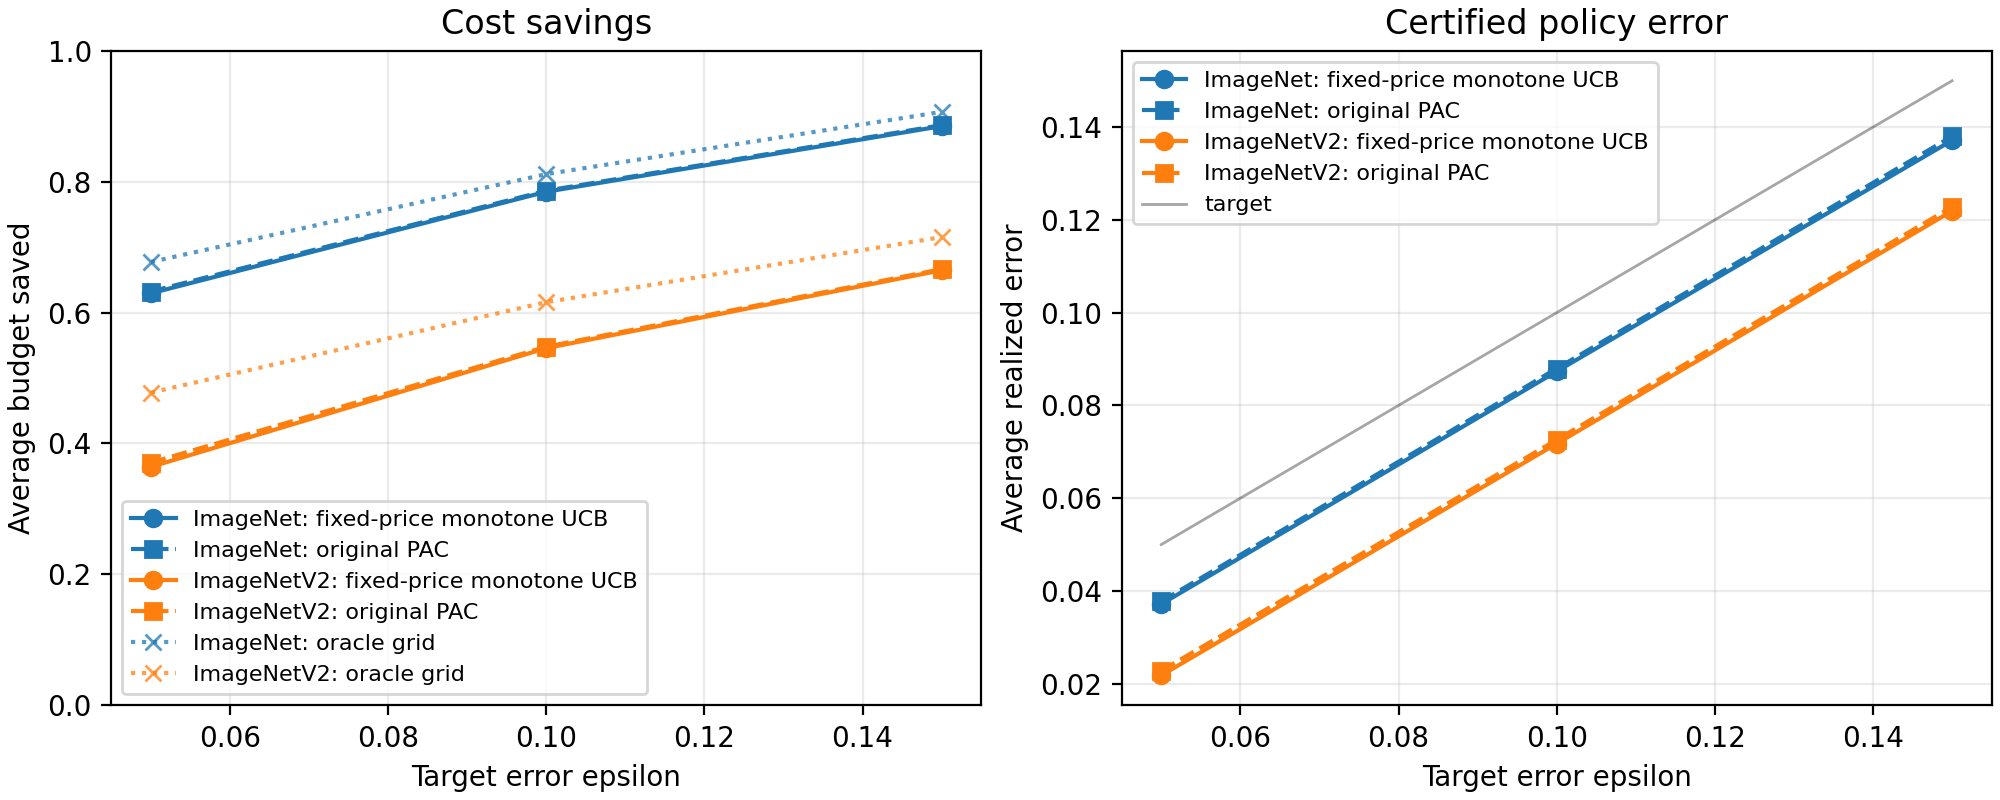
\includegraphics[width=0.95\textwidth]{results/simple_offline_pac/simple_offline_pac_summary.png}
\caption{Offline sweep over target error levels. The fixed-price UCB rule is
more conservative than the original scalar PAC baseline in this single-source
experiment, but both maintain zero empirical violation over 500 trials.}
\label{fig:offline-main-results}
\end{figure}

\paragraph{Online audited routing.}
The online experiment uses a random stream order and the dual-price update in
Section~3 with audit probabilities $p\in\{0.1,0.2,0.5\}$.
These runs set the internal online target to $\eps_0=\eps$, so they are a
behavioral check of the audited update rather than a theorem-tight
slack-adjusted implementation of Corollary~\ref{cor:online-pac-tuning}.
Lower audit rates save more expert budget but leave less correction, so final
error is closer to the target.
At $\eps=0.10$, ImageNet has no final-error violations for all three audit
rates; ImageNetV2 has a small violation rate at $p=0.1$ and none at
$p\ge0.2$.

\begin{table}[H]
\centering
\small
\begin{tabular}{lccccc}
\toprule
Dataset & $p$ & Final error & AI error & Violation & Budget saved \\
\midrule
ImageNet & 0.1 & 0.0760 & 0.0844 & 0.0000 & 0.6560 \\
ImageNet & 0.2 & 0.0725 & 0.0906 & 0.0000 & 0.6076 \\
ImageNet & 0.5 & 0.0488 & 0.0976 & 0.0000 & 0.3945 \\
ImageNetV2 & 0.1 & 0.0845 & 0.0939 & 0.0260 & 0.5029 \\
ImageNetV2 & 0.2 & 0.0774 & 0.0969 & 0.0000 & 0.4645 \\
ImageNetV2 & 0.5 & 0.0497 & 0.0993 & 0.0000 & 0.3001 \\
\bottomrule
\end{tabular}
\caption{Online audited results at $\eps=0.10$.  ``AI error'' is the
counterfactual average error of AI-labeled items before audit correction;
``Final error'' is after audited items are corrected by the expert.}
\label{tab:online-main-results}
\end{table}

\section{Related Work}

\paragraph{PAC labels and conformal calibration.}
The closest starting point is PAC labeling
\cite{candes2025paclabels}, which gives finite-sample guarantees for
cost-effective dataset labeling using AI predictions and expert audits.
That framework already includes both scalar-threshold PAC labeling and
multi-model PAC routing variants.
Our formulation is best viewed as a complementary optimization-first
presentation: we start from a finite-pool cost-minimization LP, derive the
fixed-price routing rule from its dual, allow item- and source-specific costs,
and then use calibration only to certify the actual loss of the selected
proxy-generated policy.
The calibration logic is closely related to conformal prediction and
distribution-free uncertainty quantification
\cite{vovk2005,angelopoulos2021gentle}, but the object being controlled here is
the average error of a released labeled dataset rather than coverage of
prediction sets.

\paragraph{Online conformal prediction with partial feedback.}
Adaptive and online conformal methods update calibration parameters over time
to handle changing environments \cite{gibbs2021adaptive}.
Recent work has studied intermittent or semi-bandit feedback, where labels are
not always observed \cite{ge2024stochastic,wang2025mirror,yang2026adversarial}.
Those papers motivate the audited online extension in
Section~\ref{sec:online-audited}: when labels are not always revealed, the
feedback used to update a calibration or price parameter must be corrected for
the observation process.

\paragraph{Learning to defer and cost-sensitive routing.}
Learning-to-defer methods train systems that either predict or pass an item to
an expert \cite{madras2018predict,mozannar2020consistent}.
Multiple-expert and cost-sensitive variants study richer deferral and routing
settings \cite{mao2023twostage,alves2024cost}.
The distinction here is the finite-sample PAC certificate for the final
released labels.
The proxy router may be learned by standard supervised methods, but the
guarantee comes from held-out calibration of the actual selected policy.

\section{Discussion}

The report separates two regimes.
The offline method has a clean division of labor.
The proxy model and the LP structure make the policy cost efficient; the
calibration set makes it valid.
When instantiating the method, the main modeling choice is whether the target
is transductive or inductive.
If the application is dataset curation for a fixed unlabeled pool, the
transductive theorem should be the main result.
If the application is repeated deployment on future items, the inductive
statement should be foregrounded.
The online method addresses a different obstacle: the selected policy changes
over time and AI losses are not observed without expert reveal.
Random audits supply the missing feedback through an inverse-probability loss
estimate.
This gives finite-horizon error control, but not a cost-regret comparison to
the offline oracle LP.
The experiments in Section~\ref{sec:experiments} illustrate this distinction:
offline calibration gives a clean finite-policy certificate, while the online
mechanism exposes an explicit audit-cost versus correction tradeoff.
The main empirical limitation is that the current data contain only one cheap
source.
A stronger test of the LP perspective would use several cheap sources with
heterogeneous costs, where the original scalar threshold structure no longer
captures the routing problem.

\appendix

\section{Proofs}
\label{app:proofs}

\paragraph{Proof of Proposition 1.}
The derivation in Section~\ref{sec:optimization-dual} gives the Lagrangian
\eqref{eq:full-lagrangian}.
Taking the infimum over $x_{t,a}\ge0$ yields the dual feasibility constraints
\eqref{eq:dual-feasibility-mu} and hence the explicit dual
\eqref{eq:explicit-mu-dual}.
Eliminating $\mu_t$ gives \eqref{eq:dual-problem}.
The primal is feasible because choosing the expert for all items gives zero
loss, and it is bounded because costs are nonnegative and finite.
Therefore strong duality holds by finite-dimensional linear programming
duality.
For the support statement, complementary slackness for the primal variable
$x_{t,a}$ implies that $x_{t,a}>0$ only when
\[
    \mu_t
    =
    \frac1T\{C_t(a)+\lambda h_t(a)\}.
\]
At a dual optimum, $\mu_t$ is the minimum feasible upper bound over actions,
so this equality can hold only for actions minimizing
$C_t(a)+\lambda h_t(a)$.
The deterministic optimality claim is then the standard complementary-slackness
condition for the global risk constraint. \hfill$\square$

\paragraph{Proof of Lemma 1.}
At an extreme point, the number of positive variables is at most the number of
linearly independent active equality constraints after converting the active
global risk constraint, if any, to an equality.
There are $T$ row-sum constraints and at most one active global risk
constraint, so an extreme point has at most $T+1$ positive variables.
Every row $t$ must have at least one positive variable because
$\sum_a x_{t,a}=1$.
Thus at most one row can contain more than one positive variable.
Rounding only that row changes one term in the loss average and one term in the
cost average, giving the stated bounds. \hfill$\square$

\paragraph{Proof of Theorem 1.}
For each fixed $\lambda\in\Lambda$, the variables
$H_{I_s}(\lambda)$ are i.i.d. in $[0,1]$ with mean $L_T(\lambda)$ conditional
on the target pool.
Hoeffding's inequality gives
\[
    \Pp\left\{
        L_T(\lambda)>
        \hatL_m(\lambda)+
        \sqrt{\frac{\log(|\Lambda|/\alpha)}{2m}}
    \right\}
    \le \frac{\alpha}{|\Lambda|}.
\]
A union bound over $\Lambda$ implies that, with probability at least
$1-\alpha$,
\[
    L_T(\lambda)\le U_m(\lambda;\alpha)
    \qquad \text{for every }\lambda\in\Lambda.
\]
On this event, the selected price satisfies
\[
    L_T(\hat\lambda)
    \le U_m(\hat\lambda;\alpha)
    \le \eps
\]
by construction.
The final label loss equals $H_t(\hat\lambda)$ on items not corrected by the
expert and is at most $H_t(\hat\lambda)$ on calibration items if they are
released with their expert labels.
This proves the claim. \hfill$\square$

\paragraph{Proof of Corollary 1.}
For each fixed $\lambda\in\Lambda$, the calibration losses are i.i.d. in
$[0,1]$ with mean $L(\lambda)$.
Hoeffding's inequality and a union bound over $\Lambda$ imply that, with
probability at least $1-\alpha$ over the calibration sample,
\[
    L(\lambda)\le U_m(\lambda;\alpha)
    \qquad\text{for every }\lambda\in\Lambda.
\]
On this event, the selected price satisfies
$L(\hat\lambda)\le U_m(\hat\lambda;\alpha)\le\eps$.
Conditional on the calibration sample and on this event, the deployment losses
$\ell(Y_t,\tildeY_t)$ are independent, bounded in $[0,1]$, and have conditional
mean at most $L(\hat\lambda)\le\eps$.
Hoeffding's inequality therefore gives
\[
    \frac1T\sum_{t=1}^T\ell(Y_t,\tildeY_t)
    \le
    \eps+\sqrt{\frac{\log(1/\delta)}{2T}}
\]
with conditional probability at least $1-\delta$.
Combining the calibration and deployment events gives probability at least
$1-\alpha-\delta$. \hfill$\square$

\paragraph{Proof of Proposition 2.}
If $D_t=1$, then $H_t=0$ and $\widehat H_t=0$.
If $D_t=0$, then conditional on $\calG_t$ the audit draw is
Bernoulli$(p_t)$ and the loss
$\ell(Y_t,\hatY_t^{(j_t^\star)})$ is fixed.
Therefore
\[
    \E[\widehat H_t\mid\calG_t]
    =
    \E\left[
        \frac{A_t}{p_t}
        \ell(Y_t,\hatY_t^{(j_t^\star)})
        \,\middle|\,\calG_t
    \right]
    =
    \ell(Y_t,\hatY_t^{(j_t^\star)})
    =
    H_t.
\] \hfill$\square$

\paragraph{Proof of Theorem 2.}
First bound the price process.
If $\lambda_t\ge\lambda_{\mathrm{def}}$, then for every cheap source $j$,
\[
    c_{t,j}+\lambda_t\hath_{t,j}
    \ge
    c_{\min}+\lambda_{\mathrm{def}}\rho
    \ge
    c_E^{\max}
    \ge
    c_{t,E}.
\]
Thus the algorithm defers to the expert, so $D_t=1$ and
$\widehat H_t=0$.
Consequently $\lambda_{t+1}=[\lambda_t-\eta\eps_0]_+\le\lambda_t$.
If instead $\lambda_t<\lambda_{\mathrm{def}}$, then
$\widehat H_t\le1/p_{\min}$ and hence
\[
    \lambda_{t+1}
    \le
    \lambda_t+\eta/p_{\min}
    <
    \lambda_{\mathrm{def}}+\eta/p_{\min}.
\]
By induction, $0\le\lambda_t\le\Lambda_{\mathrm{on}}$ for all $t$.

Since $[x]_+\ge x$, the update gives
\[
    \lambda_{t+1}
    \ge
    \lambda_t+\eta(\widehat H_t-\eps_0).
\]
Summing over $t=1,\ldots,T$ yields
\[
    \sum_{t=1}^T \widehat H_t
    \le
    T\eps_0+\frac{\lambda_{T+1}-\lambda_1}{\eta}
    \le
    T\eps_0+\frac{\Lambda_{\mathrm{on}}}{\eta}.
\]

Let $M_t=H_t-\widehat H_t$.
By Proposition~\ref{prop:online-unbiased}, $M_t$ is a martingale difference
with respect to the audit filtration.
Moreover, $|M_t|\le1/p_{\min}$.
Azuma-Hoeffding gives, with probability at least $1-\delta$,
\[
    \sum_{t=1}^T M_t
    \le
    \frac{1}{p_{\min}}\sqrt{2T\log(1/\delta)}.
\]
Combining the last two displays gives \eqref{eq:online-H-bound}.
Finally, audit-and-correct gives $G_t\le H_t$ pointwise, which proves
\eqref{eq:online-G-bound}. \hfill$\square$

\paragraph{Proof of Corollary 2.}
Substitute the stated value of $\eps_0$ into
\eqref{eq:online-G-bound}.
The right-hand side becomes exactly $\eps$.
The positivity condition ensures that the internal target is feasible.
If $\eta\asymp T^{-1/2}$, $p_{\min}$ is constant, and the costs and proxy floor
are fixed so that $\Lambda_{\mathrm{on}}=O(1)$, then both excess terms in
\eqref{eq:online-G-bound} are $O(T^{-1/2})$. \hfill$\square$

\section{Experimental Details}
\label{app:experiments}

The experiments use the two ImageNet CSV files from the HW4 copy directory:
ImageNet has $T=50000$ items and ImageNetV2 has $T=10000$ items.
Each file contains a ground-truth label, a model prediction, and a confidence
score.
We treat the model prediction as the only cheap source and the ground-truth
label as the expert.
The proxy loss is $\hath=1-\textnormal{confidence}$, the cheap-source
deployment cost is zero, and the expert cost is one.
All experiments use 500 random trials.
The scripts are \texttt{run\_simple\_offline\_pac\_experiment.py} and
\texttt{run\_simple\_online\_pac\_experiment.py}.

\paragraph{Offline implementation.}
For the fixed-price method, the candidate threshold grid contains the
expert-only rule plus 201 evenly spaced confidence-loss thresholds between
0 and 1.
For each trial, the calibration indices are sampled independently and
uniformly from the target pool with replacement, with calibration size
$m=0.2T$.
The confidence level is $\alpha=0.05$ and
$\eps\in\{0.05,0.10,0.15\}$.
The original PAC baseline uses the same calibration sample but exploits the
monotone threshold structure, so its Hoeffding radius does not pay a union
bound over all candidate thresholds.

\begin{table}[t]
\centering
\small
\resizebox{\textwidth}{!}{%
\begin{tabular}{llcccc}
\toprule
Dataset & Method & $\eps$ & Error & Violation & Budget saved \\
\midrule
ImageNet & fixed-price UCB & 0.05 & 0.0290 & 0.0000 & 0.5898 \\
ImageNet & fixed-price UCB & 0.10 & 0.0793 & 0.0000 & 0.7645 \\
ImageNet & fixed-price UCB & 0.15 & 0.1290 & 0.0000 & 0.8705 \\
ImageNet & original PAC & 0.05 & 0.0377 & 0.0000 & 0.6323 \\
ImageNet & original PAC & 0.10 & 0.0879 & 0.0000 & 0.7864 \\
ImageNet & original PAC & 0.15 & 0.1380 & 0.0000 & 0.8866 \\
ImageNetV2 & fixed-price UCB & 0.05 & 0.0019 & 0.0000 & 0.0936 \\
ImageNetV2 & fixed-price UCB & 0.10 & 0.0534 & 0.0000 & 0.4923 \\
ImageNetV2 & fixed-price UCB & 0.15 & 0.1036 & 0.0000 & 0.6250 \\
ImageNetV2 & original PAC & 0.05 & 0.0228 & 0.0000 & 0.3706 \\
ImageNetV2 & original PAC & 0.10 & 0.0726 & 0.0000 & 0.5479 \\
ImageNetV2 & original PAC & 0.15 & 0.1228 & 0.0000 & 0.6665 \\
\bottomrule
\end{tabular}%
}
\caption{Full offline sweep. Error, violation, and budget saved are averages
over 500 trials.}
\label{tab:offline-full-results}
\end{table}

\paragraph{Online implementation.}
For each trial, the target pool is randomly permuted into a stream.
The update uses $\eta=1$, proxy floor $\rho=0.01$, and
$\lambda_1=1/\eps$.
The online routing rule uses the AI prediction when
$\lambda_t\max(1-\textnormal{confidence}_t,\rho)<1$ and otherwise defers to
the expert.
If the AI prediction is used, it is audited with probability
$p\in\{0.1,0.2,0.5\}$.
Audited AI labels are corrected by the expert before release; unaudited AI
labels are released as-is.
The reported ``AI error'' is the counterfactual average loss before audit
correction, and the reported final error is the realized loss after
correction.
As noted in Section~\ref{sec:experiments}, these runs set $\eps_0=\eps$
rather than subtracting the finite-horizon slack from
Corollary~\ref{cor:online-pac-tuning}.

\begin{table}[t]
\centering
\small
\resizebox{\textwidth}{!}{%
\begin{tabular}{lcccccc}
\toprule
Dataset & $\eps$ & $p$ & Final error & AI error & Violation & Budget saved \\
\midrule
ImageNet & 0.05 & 0.1 & 0.0434 & 0.0482 & 0.0100 & 0.5717 \\
ImageNet & 0.05 & 0.2 & 0.0394 & 0.0493 & 0.0000 & 0.5235 \\
ImageNet & 0.05 & 0.5 & 0.0248 & 0.0497 & 0.0000 & 0.3342 \\
ImageNet & 0.10 & 0.1 & 0.0760 & 0.0844 & 0.0000 & 0.6560 \\
ImageNet & 0.10 & 0.2 & 0.0725 & 0.0906 & 0.0000 & 0.6076 \\
ImageNet & 0.10 & 0.5 & 0.0488 & 0.0976 & 0.0000 & 0.3945 \\
ImageNet & 0.15 & 0.1 & 0.0978 & 0.1086 & 0.0000 & 0.7048 \\
ImageNet & 0.15 & 0.2 & 0.0950 & 0.1187 & 0.0000 & 0.6552 \\
ImageNet & 0.15 & 0.5 & 0.0674 & 0.1349 & 0.0000 & 0.4309 \\
ImageNetV2 & 0.05 & 0.1 & 0.0443 & 0.0492 & 0.1560 & 0.4123 \\
ImageNetV2 & 0.05 & 0.2 & 0.0394 & 0.0492 & 0.0080 & 0.3748 \\
ImageNetV2 & 0.05 & 0.5 & 0.0244 & 0.0489 & 0.0000 & 0.2372 \\
ImageNetV2 & 0.10 & 0.1 & 0.0845 & 0.0939 & 0.0260 & 0.5029 \\
ImageNetV2 & 0.10 & 0.2 & 0.0774 & 0.0969 & 0.0000 & 0.4645 \\
ImageNetV2 & 0.10 & 0.5 & 0.0497 & 0.0993 & 0.0000 & 0.3001 \\
ImageNetV2 & 0.15 & 0.1 & 0.1147 & 0.1275 & 0.0000 & 0.5601 \\
ImageNetV2 & 0.15 & 0.2 & 0.1096 & 0.1371 & 0.0000 & 0.5253 \\
ImageNetV2 & 0.15 & 0.5 & 0.0734 & 0.1470 & 0.0000 & 0.3451 \\
\bottomrule
\end{tabular}%
}
\caption{Full online sweep. Final error, AI error, and budget saved are
averages over 500 trials.}
\label{tab:online-full-results}
\end{table}

\section{Alternative Confidence Bounds}

The Hoeffding bound \eqref{eq:hoeffding-ucb} is simple but may be conservative.
Any valid one-sided mean upper confidence bound can be substituted.
For example, for a fixed $\lambda$, an empirical Bernstein bound gives
\begin{equation}
    U_m^{\mathrm{EB}}(\lambda;\alpha)
    =
    \hatL_m(\lambda)
    +
    \sqrt{\frac{2\hat V_m(\lambda)\log(2/\alpha)}{m}}
    +
    \frac{7\log(2/\alpha)}{3(m-1)},
\end{equation}
where $\hat V_m(\lambda)$ is the sample variance of $H_{I_s}(\lambda)$.
For a finite grid, replace $\alpha$ by $\alpha/|\Lambda|$.
Betting-based confidence sequences can also be used if the calibration stream
is reused while expanding the candidate price set.

\section{Not Very Meaningful Results}
\label{app:not-very-meaningful}

The following observation is included only to show that a continuum of prices
can be reduced to a finite policy class on a fixed finite dataset.
It is not a main contribution: the resulting confidence penalty may be larger
than that of a deliberately chosen price grid, and it does not remove the
uniform-certification cost.

\subsection{Continuous Prices and Breakpoint Enumeration}
\label{sec:breakpoints}

For each item $t$, set $\hath_t(E)=0$ and $\hath_t(j)=\hath_{t,j}$.
The action selected by a fixed price is the lower envelope of the $k+1$ lines
\[
    C_t(a)+\lambda\hath_t(a),
    \qquad a\in\{E,1,\ldots,k\}.
\]
With a deterministic tie-breaking rule, the action can change only when two of
these lines cross.

\begin{corollary}[Uniform certification over all prices]
\label{cor:all-prices}
Fix a bounded interval $[0,\lambda_{\max}]$ and include the expert-only policy
as an additional candidate.
Let $\Pi_{\lambda}$ be the fixed-price policy induced by
\eqref{eq:proxy-j-star}--\eqref{eq:proxy-action} on the union of the target and
calibration items.
The number of distinct induced policies over
$\lambda\in[0,\lambda_{\max}]$ is at most
\begin{equation}
    N_{\mathrm{br}}
    \le
    1+2(T+m)\binom{k+1}{2}.
    \label{eq:breakpoint-count}
\end{equation}
Therefore Theorem~\ref{thm:offline-fixed-price-pac} holds uniformly over all
$\lambda\in[0,\lambda_{\max}]$ after replacing $|\Lambda|$ in
\eqref{eq:hoeffding-ucb} by $N_{\mathrm{br}}$.
\end{corollary}

\begin{proof}
For a fixed item, the selected action is constant between consecutive crossing
points of pairs of lines
$C_t(a)+\lambda\hath_t(a)$.
There are at most $\binom{k+1}{2}$ pairwise crossings per item.
Across $T+m$ target and calibration items, there are therefore at most
\[
    B=(T+m)\binom{k+1}{2}
\]
crossing values, counting multiplicity.
These crossing values partition $[0,\lambda_{\max}]$ into at most $B+1$ open
intervals, and there are at most $B$ exact crossing points.
Within each open interval the entire vector of decisions on target and
calibration items is fixed.
At an exact crossing point, deterministic tie-breaking determines a single
additional policy, which may or may not coincide with one of the neighboring
interval policies.
Thus the number of distinct induced policies is at most $2B+1$.
Applying Theorem~\ref{thm:offline-fixed-price-pac} to one representative price
from each induced policy gives the result.
\end{proof}

\subsection{Explicit Cost Accounting}

This accounting is useful for implementation, but it is not central to the
statistical guarantee.
The main distinction is between deployment cost, development-label cost, and
audit or correction cost.

\paragraph{Deployment labeling cost.}
For a fixed offline price $\lambda$, the average deployment cost on the target
pool is
\begin{equation}
    C_T^{\mathrm{dep}}(\lambda)
    =
    \frac1T\sum_{t=1}^T
    \left[
        D_t^\lambda c_{t,E}
        +(1-D_t^\lambda)c_{t,j_t^\lambda}
    \right].
    \label{eq:deployment-cost}
\end{equation}
This is the cost optimized in \eqref{eq:certified-price-selection}.
If cheap predictions have already been precomputed at no marginal deployment
cost, set $c_{t,j}=0$.
If calling a model has a per-token, per-image, or per-query cost, include that
cost in $c_{t,j}$.

\paragraph{Offline development cost.}
If $m_{\mathrm{train}}$ expert labels are used to train $\hath$ and
$m_{\mathrm{cal}}$ expert labels are used to certify the fixed price, the
development cost is
\begin{equation}
    C^{\mathrm{dev}}
    =
    \sum_{i\in I_{\mathrm{train}}} c_{i,E}
    +
    \sum_{i\in I_{\mathrm{cal}}} c_{i,E}
    +
    \textnormal{cheap-source costs incurred on development items}.
    \label{eq:development-cost}
\end{equation}
This cost may be treated as sunk if the labeled development data already exist,
but it should be included when comparing end-to-end data-curation pipelines.

\paragraph{Audit-or-correction cost.}
In the offline setting, calibration labels play the role that audits play
online.
If calibration items are part of the target pool and are corrected to expert
labels in the released dataset, then there is no duplicate expert cost for
those items.
The total realized end-to-end cost can be written as
\begin{equation}
    C_T^{\mathrm{total}}(\lambda)
    =
    \frac1T\sum_{t=1}^T
    \left[
        (1-D_t^\lambda)c_{t,j_t^\lambda}
        +
        \ind{D_t^\lambda\;\textnormal{or}\;t\in I_{\mathrm{cal}}}c_{t,E}
    \right]
    + C^{\mathrm{train}}/T,
    \label{eq:total-cost}
\end{equation}
where $C^{\mathrm{train}}$ denotes expert-labeling cost used only for proxy
training and not for final target labels.
This formula separates expert labels used for final deferral from expert
labels used for statistical certification.

\paragraph{Online audit cost.}
For Algorithm~\ref{alg:online-audited}, the conditional expected round-$t$
cost under audit-and-correct is
\[
    \E[C_t\mid\calG_t]
    =
    D_t c_{t,E}
    +(1-D_t)\left(c_{t,j_t^\star}+p_t c_{t,E}\right).
\]
This identity isolates the extra expert cost paid to obtain online feedback;
it is not a cost-regret guarantee.

\section{Why Arbitrary Offline Labels Are Insufficient}
\label{app:no-free-lunch}

Without a relationship between the offline labeled data and the target pool, no
distribution-free guarantee is possible.
Suppose an offline labeled dataset shows that a cheap source is always correct,
while on the target pool the same source is always wrong.
If the learner observes no target labels, the two worlds are indistinguishable
from the target-pool covariates and cheap predictions alone.
Thus a PAC guarantee must rely on randomized target-pool labels, an i.i.d.
sampling assumption, a covariate-shift correction assumption, or a structural
assumption on the loss proxy.
This is the offline analogue of the online no-free-lunch issue under partial
feedback.

\begin{thebibliography}{99}

\bibitem{candes2025paclabels}
Emmanuel J. Cand\`es, Andrew Ilyas, and Tijana Zrnic.
\newblock Probably approximately correct labels.
\newblock \emph{arXiv preprint arXiv:2506.10908}, 2025.

\bibitem{vovk2005}
Vladimir Vovk, Alexander Gammerman, and Glenn Shafer.
\newblock \emph{Algorithmic Learning in a Random World}.
\newblock Springer, 2005.

\bibitem{angelopoulos2021gentle}
Anastasios N. Angelopoulos and Stephen Bates.
\newblock A gentle introduction to conformal prediction and distribution-free
uncertainty quantification.
\newblock \emph{arXiv preprint arXiv:2107.07511}, 2021.

\bibitem{gibbs2021adaptive}
Isaac Gibbs and Emmanuel Cand\`es.
\newblock Adaptive conformal inference under distribution shift.
\newblock In \emph{Advances in Neural Information Processing Systems}, 2021.

\bibitem{ge2024stochastic}
Haosen Ge, Hamsa Bastani, and Osbert Bastani.
\newblock Stochastic online conformal prediction with semi-bandit feedback.
\newblock \emph{arXiv preprint arXiv:2405.13268}, 2024.

\bibitem{wang2025mirror}
Bowen Wang, Matteo Zecchin, and Osvaldo Simeone.
\newblock Mirror online conformal prediction with intermittent feedback.
\newblock \emph{arXiv preprint arXiv:2503.10345}, 2025.

\bibitem{yang2026adversarial}
Junyoung Yang, Kyungmin Kim, and Sangdon Park.
\newblock Online conformal prediction with adversarial semi-bandit feedback via
regret minimization.
\newblock \emph{arXiv preprint arXiv:2604.17984}, 2026.

\bibitem{madras2018predict}
David Madras, Toniann Pitassi, and Richard Zemel.
\newblock Predict responsibly: Improving fairness and accuracy by learning to
defer.
\newblock In \emph{Advances in Neural Information Processing Systems}, 2018.

\bibitem{mozannar2020consistent}
Hussein Mozannar and David Sontag.
\newblock Consistent estimators for learning to defer to an expert.
\newblock In \emph{Proceedings of the 37th International Conference on Machine
Learning}, PMLR 119:7076--7087, 2020.

\bibitem{mao2023twostage}
Anqi Mao, Christopher Mohri, Mehryar Mohri, and Yutao Zhong.
\newblock Two-stage learning to defer with multiple experts.
\newblock In \emph{Advances in Neural Information Processing Systems}, 2023.

\bibitem{alves2024cost}
Jean V. Alves, Diogo Leit\~ao, S\'ergio Jesus, Marco O. P. Sampaio,
Javier Li\'ebana, Pedro Saleiro, M\'ario A. T. Figueiredo, and Pedro Bizarro.
\newblock Cost-sensitive learning to defer to multiple experts with workload
constraints.
\newblock \emph{Transactions on Machine Learning Research}, 2024.

\end{thebibliography}

\end{document}
